\documentclass[a4paper, 11pt]{article}
\usepackage{amsmath}
\usepackage{amsfonts}
\usepackage{amssymb}
\usepackage{caratula}
\usepackage[spanish, activeacute]{babel}
\usepackage[usenames,dvipsnames]{color}
\usepackage[width=15.5cm, left=3cm, top=2.5cm, height= 24.5cm]{geometry}
\usepackage{graphicx}
\usepackage[utf8]{inputenc}
\usepackage{listings}
\usepackage[all]{xy}
\usepackage{multicol}
\usepackage{subfig}

\usepackage{cancel}
\usepackage{float}
\usepackage{xcolor}
\usepackage{color,hyperref}

\usepackage{multirow} % para las tablas


%%%%%%%%%%%%%% ALGUNAS MACROS %%%%%%%%%%%%%%
% For \url{SOME_URL}, links SOME_URL to the url SOME_URL
\providecommand*\url[1]{\href{#1}{#1}}

% Same as above, but pretty-prints SOME_URL in teletype fixed-width font
\renewcommand*\url[1]{\href{#1}{\texttt{#1}}}

% Comando para poner el simbolo de Reales
\newcommand{\real}{\hbox{\bf R}}

\providecommand*\code[1]{\texttt{#1}}

%uso: \ponerGrafico{file}{caption}{scale}{label}
\newcommand{\ponerGrafico}[4]
{\begin{figure}[H]
	\centering
	\subfloat{\includegraphics[scale=#3]{#1}}
	\caption{#2} \label{fig:#4}
\end{figure}
}

%\renewcommand{\algorithmiccomment}[1]{\hfill #1}

%%%%%%%%%%%%%%%%%%%%%%%%%%%%%%%%%%%%%%%%%%%%

\materia{Ingeniería de Software II}

\titulo{Big Tiza}
%\fecha{fecha de entrega}
%\grupo{Nro grupo}
\integrante{Agustina Ciraco}{630/06}{agusciraco@gmail.com}
\integrante{Alejandro Rebecchi}{15/10}{alejandrorebecchi@gmail.com}
\integrante{Maria Lara Gauder}{27/10}{marialaraa@gmail.com}
\integrante{Martin Heredia}{146/11}{martin.herediaf@gmail.com}

\include{templates}

\begin{document}
\pagestyle{myheadings}
\maketitle
%\markboth{Nombre materia}{Nombre TP}

\thispagestyle{empty}
\tableofcontents

%\setcounter{section}{-1}
\newpage

\section{Introducci\'on}

En este trabajo práctico se presentan las arquitecturas del sistema correspondiente a la primera entrega (versión para escuela de villa urquiza) y la correspondiente al sistema pedido por el ministro, cuyo alcance es a nivel pais.
Se detallan los atributos de calidad pedidos, junto con sus respectivos escenarios. Por otro lado se presenta una discusión sobre las diferencias entre las metodologías utilizadas en cada tp, y por último conclusiones.
\newpage
\section{Atributos de Calidad}
\subsection{Listado atributos de calidad pedidos}
\begin{itemize}
\item[Performance] Monitorear el estado de las campañas de manera agil. No se admiten demoras de ningún tipo .
Performance - Deadline
Fuente: Externa
Estímulo: El usuario desea ver el estado actual de la campaña. Requiere visualización de las estadísticas generadas hasta el momento, de los mensajes enviados y los no enviados. 
Entorno: Sobrecargado
Artefacto: Sistema
Respuesta: 
Medición de la respuesta: 

\item[Disponibilidad] Fallas de comunicación durante transición de servidores

\textbf{Fuente}: 
\textbf{Estímulo}:
\textbf{Entorno}: 
\textbf{Artefacto}: 
\textbf{Respuesta}: 
\textbf{Medición de la respuesta}: 

\item[Modificabilidad] Cambio de servidores entre etapa de Cordoba a etapa pais.

\textbf{Fuente}:  \\
\textbf{Estímulo}: \\
\textbf{Entorno}: \\
\textbf{Artefacto}: \\
\textbf{Respuesta}: \\
\textbf{Medición de la respuesta}: \\


\item[Seguridad]Proteger datos y modificación (campañas y evaluación).

\textbf{Fuente}:  \\
\textbf{Estímulo}: \\
\textbf{Entorno}: \\
\textbf{Artefacto}: \\
\textbf{Respuesta}: \\
\textbf{Medición de la respuesta}: \\

\item[Seguridad]Auditar


\textbf{Fuente}:  \\
\textbf{Estímulo}: \\
\textbf{Entorno}: \\
\textbf{Artefacto}: \\
\textbf{Respuesta}: \\
\textbf{Medición de la respuesta}: \\

\item[Disponibilidad] Envio de mensajes. (Patagonia)


\textbf{Fuente}:  \\
\textbf{Estímulo}: \\
\textbf{Entorno}: \\
\textbf{Artefacto}: \\
\textbf{Respuesta}: \\
\textbf{Medición de la respuesta}: \\


\item[Certeza de Datos] Para la estimacion de campanias

\textbf{Fuente}:  \\
\textbf{Estímulo}: \\
\textbf{Entorno}: \\
\textbf{Artefacto}: \\
\textbf{Respuesta}: \\
\textbf{Medición de la respuesta}: \\

\item[Modificabilidad-Scalabilidad] Volumen de datos


\textbf{Fuente}:  \\
\textbf{Estímulo}: \\
\textbf{Entorno}: \\
\textbf{Artefacto}: \\
\textbf{Respuesta}: \\
\textbf{Medición de la respuesta}: \\

\item[Performance-Escalabilidad] Mantener el 80 porciento de tiempo de envio.

\textbf{Fuente}:  \\
\textbf{Estímulo}: \\
\textbf{Entorno}: \\
\textbf{Artefacto}: \\
\textbf{Respuesta}: \\
\textbf{Medición de la respuesta}: \\

\item[Modificabilidad] Campanias privadas
A futuro se quiere poder permitir a empresas privadas crear campañas con de promoción de p
\textbf{Fuente}:  
\textbf{Estímulo}: \\
\textbf{Entorno}: \\
\textbf{Artefacto}: \\
\textbf{Respuesta}: \\
\textbf{Medición de la respuesta}: \\

\item[Flexibilidad] politica nacional de metricas
\textbf{Fuente}:  \\
\textbf{Estímulo}: \\
\textbf{Entorno}: \\
\textbf{Artefacto}: \\
\textbf{Respuesta}: \\
\textbf{Medición de la respuesta}: \\

\item[Usabilidad] Crear campanias
Se desea que los usuarios puedan crear campañas correctamente de forma facil y rapida
\textbf{Fuente}:  Usuario
\textbf{Estímulo}: Pedido de creacion de campaña
\textbf{Entorno}: Funcionamiento normal
\textbf{Artefacto}: Aplicacion web
\textbf{Respuesta}: El usuario crea una campaña correctamente
\textbf{Medición de la respuesta}: En un test de usabilidad el 95\% de los usuarios logra crear una campaña correctamente en menos de 5 minutos

\item[Usabilidad] Visualizar campanias
Se desea poder ver toda la informacion referida a una campaña de forma clara.
\textbf{Fuente}:  Usuario
\textbf{Estímulo}: Pedido de visualizacion de campaña
\textbf{Entorno}: Funcionamiento normal
\textbf{Artefacto}: Aplicación web
\textbf{Respuesta}: Se visualiza toda la informacion disponible relacionada con la campaña
\textbf{Medición de la respuesta}: En un test de usabilidad el 95\% de los usuarios logran extraer la información esperada en menos de 30 segundos

\item[Usabilidad] Visualizar Resultados
Se desea poder comparar resultados de varias campañas de forma comparable, fàcil de entender.
\textbf{Fuente}: Usuario
\textbf{Estímulo}: Pedido de comparación de resultados de 2 campañas
\textbf{Entorno}: Funcionamiento normal
\textbf{Artefacto}: Aplicacion web
\textbf{Respuesta}: Se muestran los resultados de ambas campañas en la misma pantalla
\textbf{Medición de la respuesta}: En un test de usabilidad el 95\% de los usuarios logran comprender los resultados en menos de 5 minutos

\end{itemize}
\subsection{Escenarios de Atributos de calidad}
\begin{table}[H]
\centering
\begin{tabular}{ | p{5cm} | p{8cm} | p{1.5cm} | }
\hline
Clasificación & Caso de Uso & Horas H.\\ \hline \hline
\multirow{2}{5cm}{Usuarios} & Ingresando al sistema & 36 \\ \cline{2-3}
& Cargando usuario & 13 \\ \hline
\end{tabular}
\end{table}


\newpage

\section{Arquitecturas}
\subsection{Arquitectura TP1}
A partir del proyecto Aula al 2020, de los objetivos planteados y el prototipo desarrollado, se define el siguiente diagrama de arquitectura:

\centerline{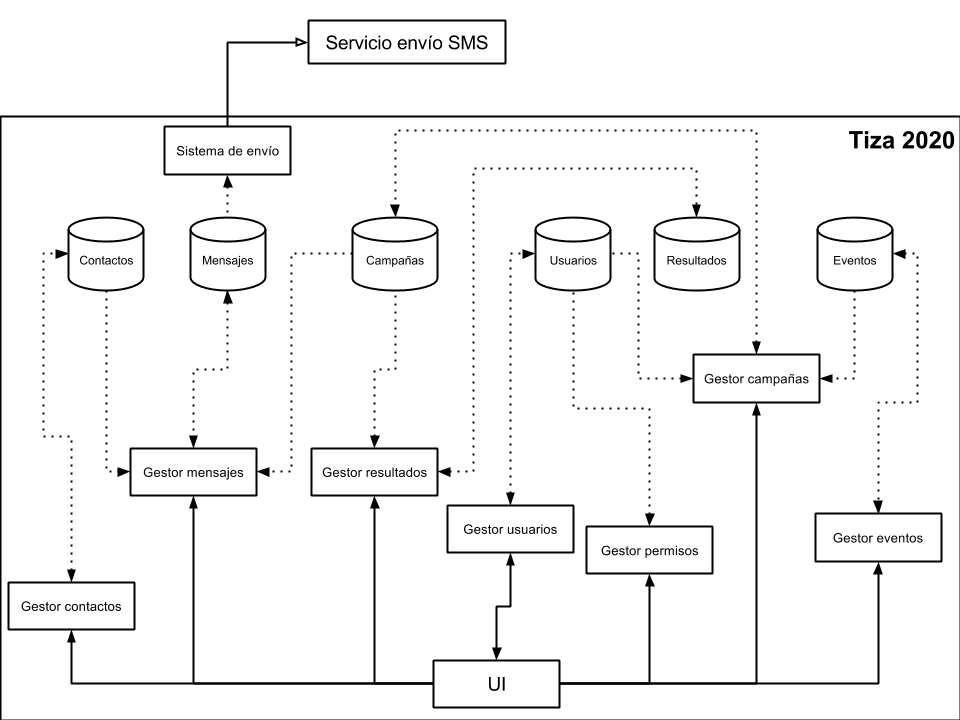
\includegraphics[width=1.2\textwidth]{./diagramas/ArquitecturaTP1.png}}
\centerline{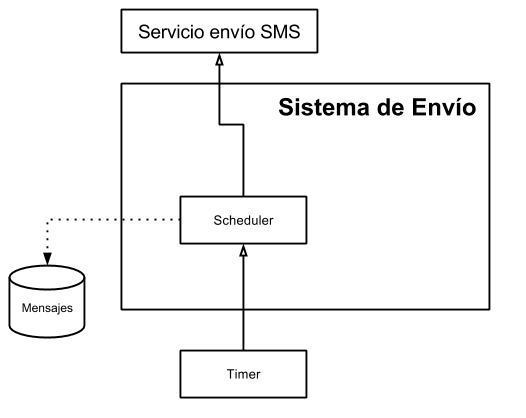
\includegraphics[width=0.5\textwidth]{./diagramas/ArqTP1SistEnvio.png}}

En primer lugar se presenta la UI, que es la encargada de la interacción del usario con el sistema de Tiza 2020. La misma recibe los pedidos por parte del usuario. Para comenzar, se deberá validar el acceso del mismo, es decir, verificar su previa inscripción en el sistema. Para eso el UI indica al \textbf{Gestor usuarios} el id del usuario que intenta acceder. Este último lee la base de datos, buscando los datos del mismo. En caso de no existir, retorna al UI un aviso de usuario inválido, el cual se encargará de notificarle a la persona. Caso contrario, responde que se permite el acceso al usuario al sistema. 
En caso de que el usuario sea válido, el UI envía un pedido al \textbf{Gestor campañas}, pidiendo las campañas correspondientes al usuario para poder mostrarlas como el siguiente menú, luego del inicio de sesión. El componente \textbf{Gestor campañas}, pide del repositorio las campañas que tienen en el campo de \emph{usuario con permiso de acceso} al id del usuario. Luego, envía la información de todas las campañas, completándolo con los datos requeridos en los demás repositorios, como podría ser el caso de los teléfonos de los contactos. 
El proceso se repite para cada menú que el usuario desee ver. Además, el gestor se encargará de recolectar la información necesaria y traducirla a una interfaz para que sea comprensible por el usuario y se le enviará al UI, quien se encarga de mostarla. En el caso de de que se desee mostrar la agenda correspondiente a un usuario, para poder incluirlo en la creación de un mensaje, el UI pedirá al \textbf{Gestor contactos}, la información necesaria. Este último se encargará de acceder a la base de datos y recolecctar los datos pedidos. El proceso es el mismo para el \textbf{Gestor mensajes}, \textbf{Gestor resultados}, \textbf{Gestor eventos}, siendo cada uno el encargado de interpretar para el UI los datos necesarios y de armar la interfaz necesaria. 

Por otro lado, cuando un usuario, tanto Docente como personal de la Secretaría o Dirección, desean crear o modificar algún objeto del sistema, lo indicarán al UI, utilizando los accesos que correspondan, y este se encargará de avisar al gestor que corresponda con el objeto. El gestor correspondiente se encargará de agregar el nuevo objeto al repositorio necesario.  En caso de que se desee modificar uno existente, también levantará de la base de datos el objeto, le aplicará la modificación indicada por el usuario y lo volverá a cargar en el repositorio. 

El \textbf{Sistema de envío} es el encargado de enviar los mensajes. El \emph{Timer} le envía cada hora un mensaje asincrónico al \emph{Scheduler} con la hora y fecha actuales. El \emph{Scheduler} se encargará de leer en la base de datos aquellos menajes que cumplan con esa hora y fecha de envío. Al obtener todos los mensajes, los traducirá para poder ser interpretados por el \textbf{Servicio envío SMS}. Este último es un sistema externo que se contratará para cumplir la función de enviar los SMS necesarios. 

\subsection{Arquitectura TP2}
\subsubsection{Vista Componentes y conectores}
La arquitectura de esta parte se realizó contemplando los atributos de calidad nombrados en la sección anterior. A continuación se muestra el diseño realizado para esta parte, seguido de un detalle de desiciones tomadas.
\begin{flushleft}
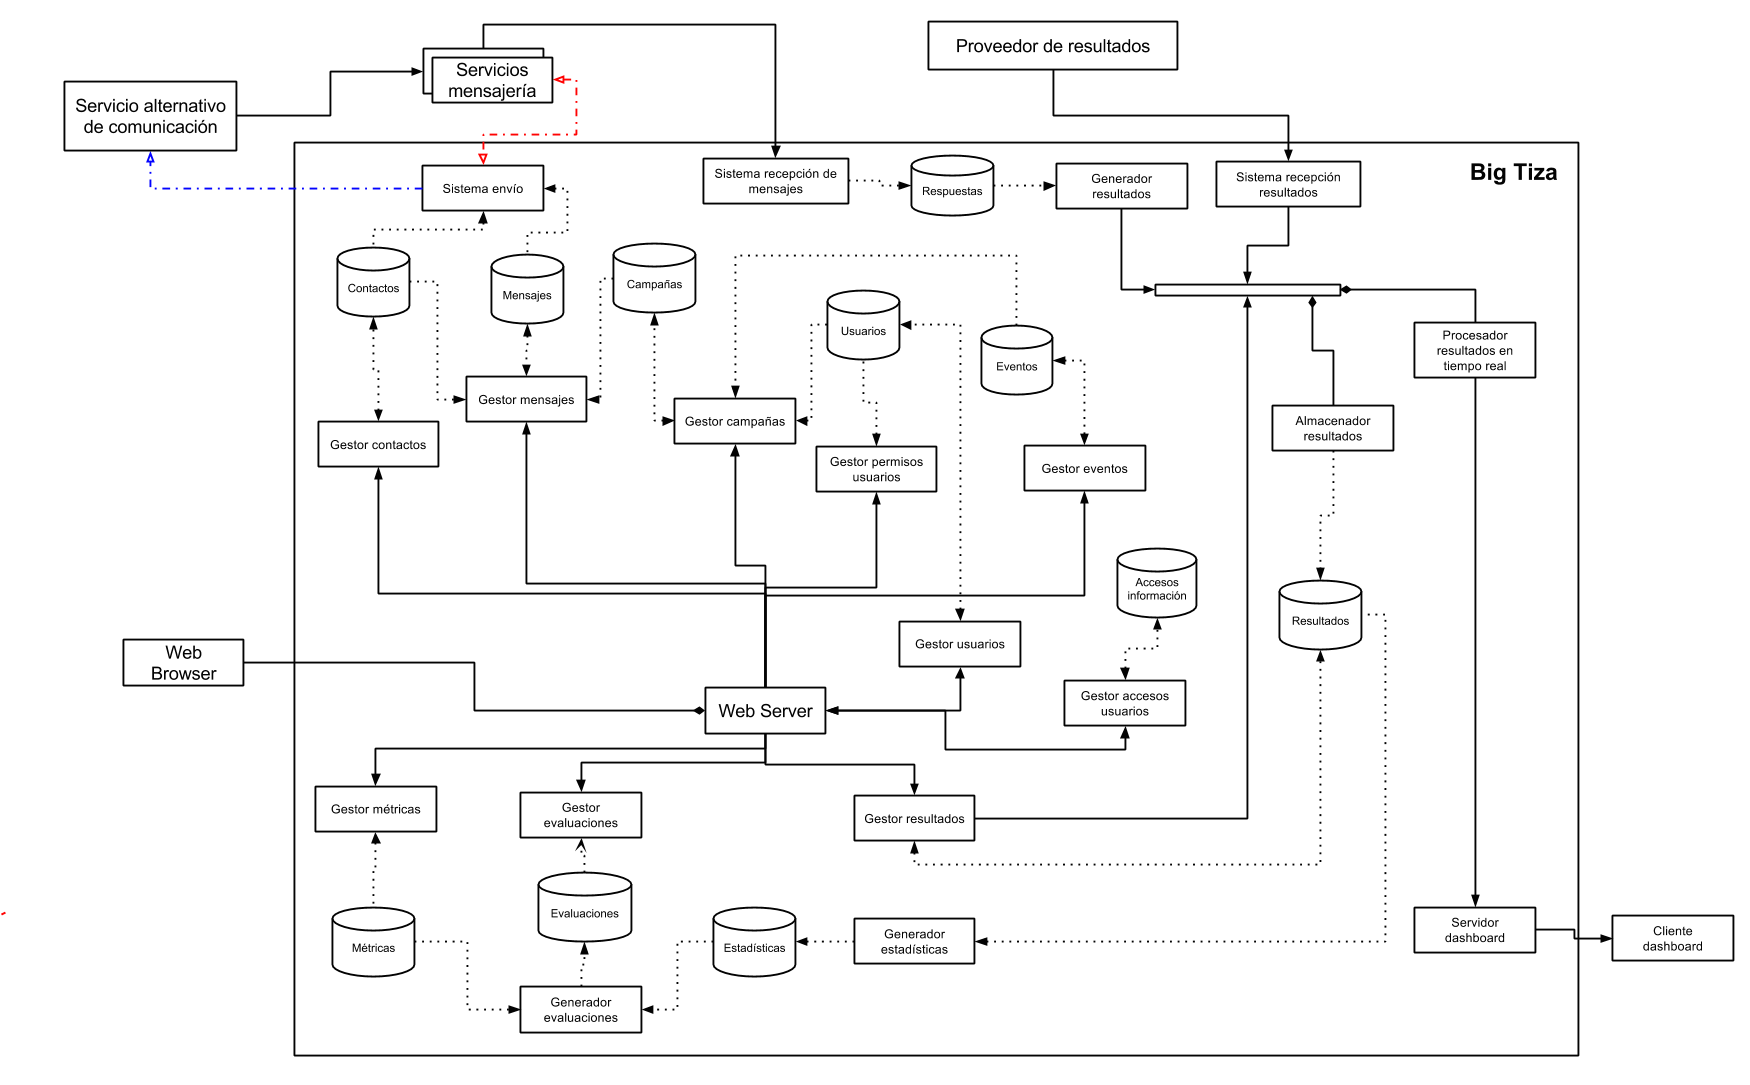
\includegraphics[width=1.3\textwidth]{./diagramas/VistaCompyCon.png}
\end{flushleft}
\emph{Desición de Diseño} Al momento de contemplar el atributo de calidad de \textbf{Disponibilidad} respecto el envío de mensajes, se tomó la decisión de realizar la conexión entre componete servicio mensajeria  y el componente, de lado de Big tiza, de envio de mensajes, mediante 2 conectores distintos. Dado que se tiene en cuenta que al momento  de enviar mensajes, puede fallar la conexión con los distintos servicios (twitter facebook, sms). 
Se optó por crear 2 conectores para esta unión, uno que muestra la conxión normal, sin fallas y otro la conexión considerando falla de comunicación.\\

\centerline{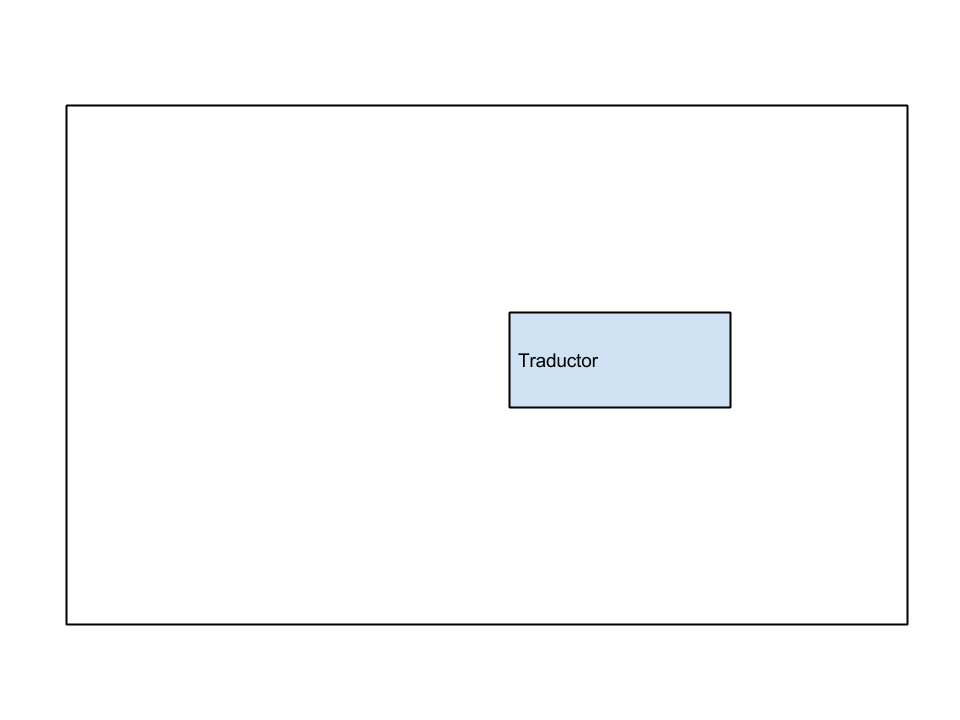
\includegraphics[width=0.6\textwidth]{./diagramas/conector_normal.png}}

Viendo en detalle el conector (1) del camino sin fallas se puede observar que existe un traductor para poder comunicarse con cada tipo de servicio (facebook, twiter etc) ya que cada uno tiene un formato distinto.
En el caso del conector (2) de camino alternativo, que contempla la falta de conexion, al ver el conector más en detalle se puede observar  que se tiene el componente servicio alternativo de mensajería, quién se encarga de tomar la decición correspondiente y conectarse con el servicio de la empresa de telefonia privada para poder concretar el envío.\\

%revisar que decision tomamos respecto a la version de oca
Además en este caso se contempló un tercer caso que coincide con el análisis de riesgo, tomado para la parte de planificación, donde se considera una conexión directa con un servicio de correo (oca), para poder contar con él en el caso de no tener ningún tipo de conexión con los otros servicios.\\ %de esa manera se desliga el sistema Big tiza de esa responsabilidad.

Al considerar las situaciones de envío de camino sin fallas, donde como hay que evitar el uso de la empresa de telefonía privada, ya que esta puede generarle costos a los receptores, lo cual se desea evitar, por lo que se van a hacer varios intentos, antes de tomar la desición de cambiar de conector.\\
\\
\\
%~ Para la decision de por donde enviar se la asigna a un componente dentro de componente de envio de mensajes, esto se pude observar al hacer zoom de este comp 
\emph{Desicisión de Diseño}
Al momento de contemplar en las respuestas de aquellas campañas que esperar respuestas a los mensajes enviados, se asume que los mensajes se envían con un código para vincular con dicha campaña, para de esta manera poder generar los resultados correspondientes.\\

Por otro lado, se optó por tener un componente \textbf{Servicio de evaluacion de estadisticas}, el cual es externo con el cual hay que conectarse al momento de evaluar los resultados, el mismo es definido por cada municipio acorde a lo que se desee evaluar (campaña de saludo, de educacion vial, etc)\\
\\
\\
Otra parte importante a la hora de hablar de la arquitectura de Big Tiza, es la parte del procesado de resultados de las campañas, ya que esta parte involucra 2 partes importantes, la de procesado de campañas y la parte de visualizarlos en por ejémplo un dashboard.
En cuando al procesado de los resultados, primero hay que considerar cómo llegan al sistema, una opción posible es la carga manual de dichos resultado. Esta opción es considerada dado que hay campañas, como por ejemplo una campaña de vacunación, que requiere de requiere de un proceso de que la misma llegue a la población, se considere y tenga efecto, en este ejémplo el efecto es que la persona se vacune y cuando lo haga eso suma un resultado a la campaña,como que 100 personas recibieron la vacuna para la gripe en el hospital de villa urquiza el día 4 de mayo de 2015, que luego será agregado al sistema por personal reponsable.
Respecto a la arquitectura considerada para este punto, quién recibe los resultados dichos anteriormente es el componente gestor de resultados.
Por otro lado, se contemplan campañas interactivas, es decir que envían mensajes cuyo efecto es una respuesta el mensaje envíado, por lo cual este tipo de resultados, se reciben directamente en el sistema, el encargado de recibirlo nuevamente es el componente gestor de resultados.\\
\\
\\
Al recibir un resultado de una campaña, éste debe ser procesado inmediatamente para poder ser visualizado lo antes posible, ya que se desea obterner el dashboard siempre actualizado (el dashboard es el componente que se encargará de contemplar el requerimiento de que las campañas se puedan monitorear de manera ágil). por ejémplo se puede considerar el resultado 4 personas recibieron la vacuna contra la gripe en el hospital Posadas, estos valores deben ser evaluados acorde a las métricas definidas para la campaña definida por el ministerio de salud para la prevención de la gripe. Dependiendo de la definición de la métrica este valor (4 personas) puede ser bueno o malo. ya que por ejémplo si se espera que haya 100 personas vacunadas en el posadas, este valor es bajo. Luego de evaluar dicho resultado, el mismo está listo para ser visualizado en el dashboard, también se guarda para una vez que se haya finalizado la campaña el mismo pueda ser reunido con todos los resultados de la misma y obtener así un resultado final certero de la campaña.\\
\\
\\
Otro aspecto que fue considerado al momento de definir la interfaz para que un usuario pueda definir campañas es el de seguridad, ya que se hizo hincapié en que van a haber distintos tipos de usuario, y no todos pueden ver información de todas las campañas, en particular a la hora de tener la posibilidad de agregar campañas para empresas privadas, como por ejémplo addidas, se quiere tener la posibilidad de restringir la información a la que accede el usuario representante a addidas.
\emph{Desición de diseño} Para cubrir este requerimiento se decidió agregar un web browser. \\
\\
\\
Otras consideraciones que se tienen respecto de la seguridad de la información, es que los otros canales de acceso al sistema, por ejémplo la carga de resultados, o como el componente de recepción de mensajes, tengan revisiones de seguridad previo a acceder a la base de datos para persistir información, para evitar un potencial ataque de seguridad.\\
\\
\\s
Volviendo al requerimiento de visualizar el resultado de campañas de manera ágil, como se presento anteriormente, se consideró un dashboard.
\emph{Desición de diseño} Para ello se optó por realizar un componente \textbf{Servidor Dashboard} el cual se responsabiliza de recibir y mostrar los resultados, constantemente. Además este componente tiene dos formas de recibir resultados. Dado que se desea optener en tiempo real resultados procesados una forma de que el componente reciba es el camino de los valores que se evaluan constantemente de la campaña, y otra es cuando se tienen resultados finalizados de las misma los puede seguir visualizando a pedido del componente \textbf{Cliente Dashboard} del lado del usuario.\\
\\
\\
Se tomó esta decisión teniendo en cuenta el volumen de información a procesas y los recursos con los que se cuentan, ya que durante la vigencia de una campaña se van a obtener volumenes muy grandes de resultados parciales,  que los mismos se quieren ver reflejados en el dashboard, pero también se desea tener la información correcta del resultado final conseguido a través de la campaña concretada. Al considerar resultados parciales se desea conseguir valores representativos al volumen total de insidencia de la campaña, por lo que esos resultados parciales se deben evaluar a nivel porcentaje de insidencia de dicho volumen para que al visualizar se pueda reflejar la métrica utilizada por la campaña.
Teniendo en cuenta los escenarios de performance se tomó la desición dicha anteriormente.

\subsubsection{Vista Alocación}

\centerline{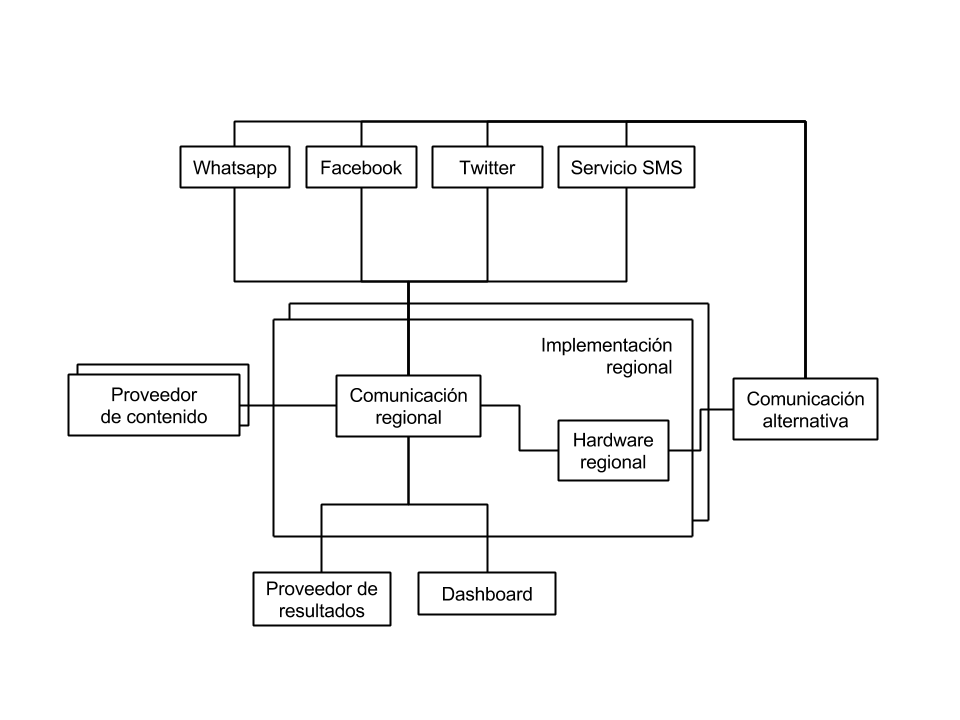
\includegraphics[width=0.6\textwidth]{./diagramas/VistaAlocacion.png}}

En esta vista se muestran dónde está contenido cada componente externo presentado en la vista anterior. En este diagrama se puede observar que los servicios de mensajería se separan y muestran cada uno en particular, ya que se considera que cada servicio corre por separado ya que son empresas diferentes.\\
\\
Por otro lado se muestran los proveedores de contenido que es aquel componente responsable de agregar a las campañas aquellos logos, mensajes o lo que se desee mostrar, esto se decidió en consideración a que las campañas, tanto en esta primer etapa como en la siguiente, van a ser de distintas índoles ya sea para creación de una campaña por el ministerio de salud, como por el ministerio de seguridad vial, y en particular en un futuro se consideran las campañas de empresas privadas como NIKE.\\
\\
Por último, se puede destacar el componente \textbf{Empresa de telecomunicaciones} a quién se le asigna en el conector de camino con falla de conexión, la responsabilidad de enviar los mensajes utilizando su infraestructura, por ello dicho sistema está por fuera de Big Tiza.


%~ \subsection{Discusión de Arquitecturas}

\newpage
\section{Discusión}

\newpage
\section{Conclusiones}

\subsection{Programming in the Large vs Programming in the Small}

En esta secci\'on se comparar\'an la Arquitectura correspondiente al Dise\~no Orientado a Objetos (small programming) y la nueva Arquitectura de gran escala (large programming) correspondientes a este trabajo.

{\bf Comunicaciones con entidades externas} \\
\begin{tabular}{| p{8cm} | p{8cm} |}
\hline
Dise\~no O. O. & Arquitectura \\ \hline \hline
Un solo componente externo, correspondiente al Sitema de Env\'io de Mensajes. Esto se debi\'o a que era el \'unico canal de comunicaci\'on. Con respecto a los resultados, estos eran cargados manualmente al sistema. & La cantidad de canales de comunicaci\'on aumentaron, no s\'olo abarcando al anterior Sistema de Envio de Mensajes, sino tambi\'en a redes sociales como Facebook y Twitter, y la posibilidad de env\'io por Correo Argentino. Para los resultados, como la cantidad de mensajes y respuestas son masivas, hacerlo manualmente ser\'ia imposible. Para esto se cuenta con la opci\'on de poder ser cargadas autom\'aticamente por medio de Web Services externos (como por ejemplo, un Web Service ofrecido por el Ministerio de Salud, para obtener resultados de campa\~nas de salud) \\ \hline
\end{tabular}


{\bf Seguridad de datos} \\
\begin{tabular}{| p{8cm} | p{8cm} |}
\hline
Dise\~no O. O. & Arquitectura \\ \hline \hline

La comunicaci\'on con el sevicio de Mensajer\'ia SMS era insegura. Cualquier persona podr\'ia capturar el tr\'afico y obtener datos privados de los usuarios. & Ahora nuestro sistema al ser a escala Provincial (y posteriormente a escala Nacional), debe garantizar la seguridad de los datos de cada usuario. Esto se logra por medio de algortimos de encriptaci\'on. \\ \hline
\end{tabular}


{\bf Disponibilidad} \\
\begin{tabular}{| p{8cm} | p{8cm} |}
\hline
Dise\~no O. O. & Arquitectura \\ \hline \hline

No siempre estaba garantizado que los mensajes enviados efectivamente llegaran. Si luego de 3 intentos no se lograba enviar algun mensaje, se lo descartaba. & Para intentar suplir la anterior falla, los mensajes persisten en el tiempo, y mientras tenga sentido el mensaje en el contexto de su campa\~na y a\'un no haya llegado, se prueba el env\'io por otros medios previamente mencionados o se reenintenta en caso de haber ya agotado todos los canales posibles. \\ \hline
\end{tabular}

{\bf Alocaci\'on} \\
\begin{tabular}{| p{8cm} | p{8cm} |}
\hline
Dise\~no O. O. & Arquitectura \\ \hline \hline

Al no ser muy grande el sistema y la cantidad de datos no era demasiada, con una m\'aquina alcanzaba para alocar cada componente del mismo y almacenar las campa\~nas, mensajes, usuarios y destinatarios. & Ahora aparece el conceto de BigData. Se cuenta con una masiva cantidad de datos y a la vez est\'a la necesidad de implementar sistemas performante. Es por esto que ahora el sistema esta alocado en varios servidores, aprovechando la capacidad de paralelizar trabajo y distribuir estrat\'egimante los datos entre todos estos lugares. \\ \hline
\end{tabular}


{\bf T\'acticas} \\
\begin{tabular}{| p{8cm} | p{8cm} |}
\hline
Dise\~no O. O. & Arquitectura \\ \hline \hline

En esta arquitectura no se ven reflejadas ninguna de las t\'acticas de atributos de calidad, ya que no fueron tenidas en cuenta. & Se vi\'o en la necesidad de aplicaci\'on de algunas t\'acticas para la resoluci\'on de problemas t\'ipicos de Disponibilidad, Performance, Seguridad entre otros. \\ \hline
\end{tabular}


{\bf Big Data} \\
\begin{tabular}{| p{8cm} | p{8cm} |}
\hline
Dise\~no O. O. & Arquitectura \\ \hline \hline

Como se mencion\'o previamente, en esta etapa la cantidad de datos es m\'inima, con lo cual esto permit\'ia que para poder obtener el estado de todas las campa\~nas, con un simple listado de las mismas se lograba visualizarlas, y no se consum\'ia mucho tiempo. & En cambio, y como tambi\'en se mencion\'o, en esta etapa al haber una inmensa cantidad de datos, la visualizaci\'on de las campa\~nas pasa a ser un reto. Aparece la necesidad de aplicar heur\'isticas usando estad\'isticas para dar una idea del estado de las mismas, debido a la imposibilidad de brindar un servicio exacto tiempo real. \\ \hline
\end{tabular}

\end{document}
